\documentclass{article}
\usepackage[utf8]{inputenc}
\usepackage[T1]{fontenc}
\usepackage[top=2cm,bottom=2cm,left=3cm,right=3cm]{geometry}
\usepackage{hyperref}
\usepackage{amsmath,amsfonts,amssymb,amsthm}
\usepackage{graphicx}
\usepackage[dvipsnames]{xcolor}

\renewcommand{\figurename}{Rysunek}


\begin{document}
	\title{ \LARGE \textsc{Bazy danych}
		\\ [5.5cm]
		\huge \textbf{\uppercase{Baza danych Geeks \& Dragons}}
		\\ [0.5cm]
		\large \textbf{\uppercase{Dokumentacja}}
		%\\ [0.5cm]
		%\normalsize \today \vspace*{20\baselineskip}
		}
	\date{}
	\maketitle
	\vspace{7.5cm}
	
	\begin{center}
	\author{
		Szymon Malec, 262276 \\
		Adam Wrzesiński, 262317\\
		Michał Wiktorowski, 262330 \\
		Weronika Zmyślona, 262284 \\
		\vspace{0.5cm}
		Politechnika Wrocławska \\
		Wydział Matematyki - Matematyka Stosowana}
	\end{center}
	
	\thispagestyle{empty}
	
	\newpage\thispagestyle{empty}
	\mbox{}
	
	\setcounter {page}{1}
	
	\tableofcontents
	
	\newpage
	\section{Wstęp}
	Niniejsza dokumentacja przedstawia proces tworzenia bazy danych sklepu Geeks \& Dragons w ramach projektu na zaliczenie z kursu Bazy Danych z 2023 roku. Zadanie polegało na wysymulowaniu danych, jakie mogłyby się pojawić w bazie przykładowego sklepu, mającego w ofercie gry nieelektroniczne, który dodatkowo prowadzi wypożyczalnię gier oraz organizuje turnieje. Projekt został wykonany z~wykorzystaniem języka programownaia Python.\\
	
	Pierwszą częścią projektu było wykonanie schematu bazy danych, a następnie wygenerowanie losowych danych. Uzyskane dane należało eksportować do bazy i umieścić na serwerze za pomocą MySQL. Kolejna część polegała na przeprowadzeniu analizy danych z wysymulowanego zbioru i~przedstawienie jej w formie raportu. Ponadto został opisany przebieg normalizacji bazy danych do postaci EKNF. 
	
	\section{Schemat bazy danych}
	Schemat bazy danych (Rysunek 1.) uwzględnia 8 tabel przechowujących nastepujące informacje:
	\begin{itemize}
		\setlength{\itemsep}{-2pt}
		\item \textbf{cusomer} – dane dotyczące klientów sklepu,
		\item \textbf{staff} – dane dotyczące pracowników sklepu,
		\item \textbf{games\textunderscore for\textunderscore sale} – dane dotyczące gier dostępnych na sprzedaż,
		\item \textbf{games\textunderscore to\textunderscore rent} – dane dotyczące gier dostępnych do wypożyczenia,
		\item \textbf{sale} – dane na temat sprzedaży gier,
		\item \textbf{rental} – dane na temat wypożyczeń gier,
		\item \textbf{competition} – dane dotyczące organizownych turniejów,
		\item \textbf{competition\textunderscore results} – dane dotyczące osiągnietych wyników przez uczestników turniejów.
	\end{itemize}
	
	\begin{figure}[!h]
		\centering
		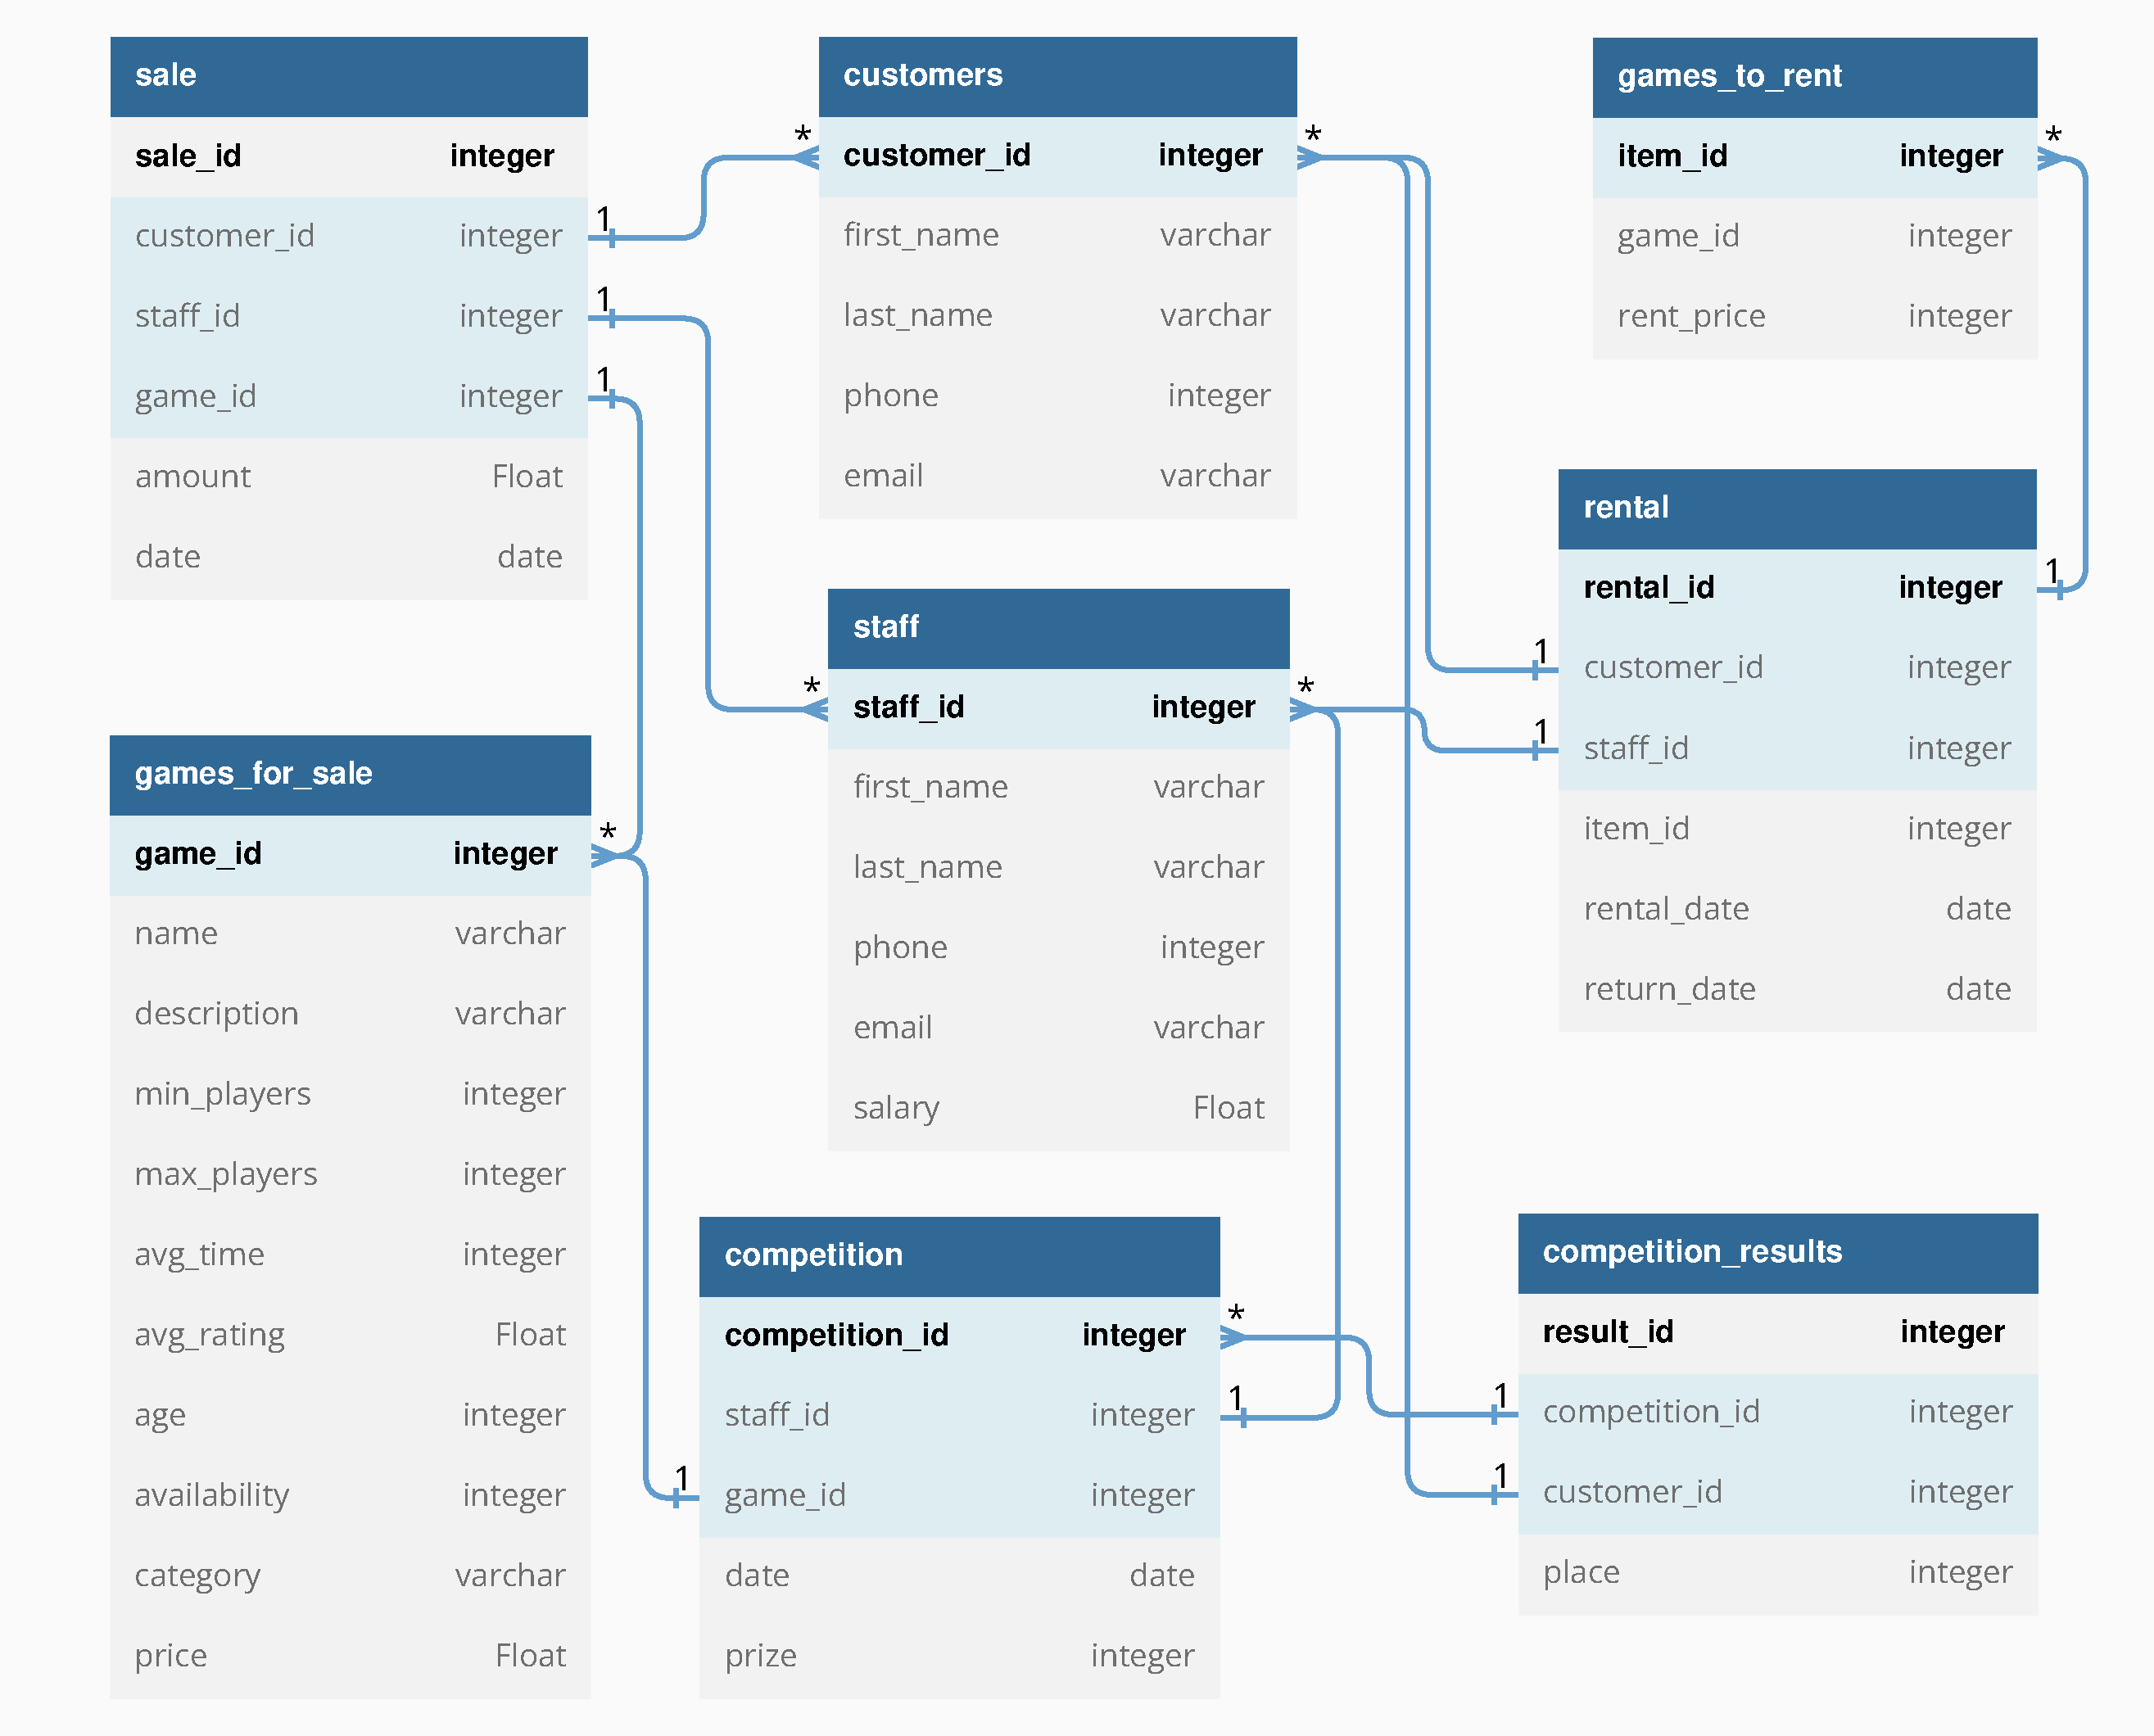
\includegraphics[width=13cm]{database_schema.pdf}
		\vspace{-0.6cm}
		\caption{Schemat bazy danych.}
	\end{figure}

	\section{Skryptowe wypełnienie bazy}
	
	W celu przygotowania do wypełnienia bazy losowo wygenerowanymi danymi, zostały stworzone pliki csv odpowiadające poszczególnym tabelom z bazy danych. Oprócz danych generowanych losowo, pojawiają się rownież dane rzeczywiste, co zostanie opisane w dalszej części tego rozdziału. Na sam koniec, po połączniu z serwerem, dane zostały zaimportowane do bazy.
	
	\subsection{Tabela customers}
		Tabela customers zawiera informacje na temat 1329 klientów, które zorganizowane są w  5 następujących kolumnach:
		\begin{itemize}
			\setlength{\itemsep}{-2pt}
			\item \textbf{cusomer\textunderscore id} – unikalne id dla każdego klienta,
			\item \textbf{first\textunderscore name} – imię klienta,
			\item \textbf{last\textunderscore name} – nazwisko klienta,
			\item \textbf{phone} – numer telefonu klienta,
			\item \textbf{email} – adres email klienta.
		\end{itemize}
		
		Dane w tabeli zostały wygenerowane w sposób losowy. Wartości w tabeli \textbf{cusomer\textunderscore id} wygenerowane zostały na pomocą odpowiedniego przedziału  dodatnich liczb całkowitych. Imiona i nazwiska klientów zostały wylosowane z odpowiednim prawdopodobieństwem korzystając z danych zamieszczonych na stronie \href{https://stat.gov.pl/}{Głównego Urzędu Statystycznego}. W pierwszej kolejności został wygenerowany wektor określający płeć klienta, z odpowiednim prawdopodobieństwem występowania danej płci, na podstawie liczby ludności we Wrocławiu z podziałem na mężczyzn i kobiety. Następnie w zależności od płci zostały przypisane imiona i nazwiska z odpowiednich tabeli danych pobranych ze wspomnianej strony internetowej.\\
		
		Następna kolumna zawiera losowo generowane numery kontaktowe klientów. Numer w każdym przypadku składa się z połączenia losowo wybieranego wyróżnika sieci telefonicznej (2 cyfry) oraz liczby z przedziału (1000000, 9000000). Lista dostępnych wyróżników została stworzona na podstawie informacji dostępnych na stronie \href{https://pl.wikipedia.org/wiki/Numery_telefoniczne_w_Polsce}{Wikipedii}. W~ten sposób uzyskaliśmy indywidualny 9-cyfrowy numer dla każdego klienta.\\
		
		Ostatnia kolumna zawiera adresy email, dla których identyfikatory użytkownika są generowane losowo na podstawie imion i nazwisk klientów. Identyfikatory adresów email składają się przykładowo:
		\begin{itemize}
			\setlength{\itemsep}{-2pt}
			\item z połączenia imienia i nazwiska lub części nazwiska klienta,
			\item z połączenia imienia lub nazwiska i losowej liczby z przedziału (100, 10000).
		\end{itemize}
	
		Każdy adres email składa się również z domeny, która była losowana z listy domen stworzonej na podstawie rankingu najpopularniejszych serwisów pocztowych w Polsce dostępnego na stronie \href{https://interaktywnie.com/biznes/artykuly/biznes/przeglad-ktora-poczta-e-mail-jest-najlepsza-16950}{interaktywnie.com}. Oczywiście, domeny były losowane z odpowiednim prawdopodobieństwem określonym według  liczby użytkowników korzystających z wybranych serwisów pocztowych.
		
	\subsection{Tabela staff}
		Tabela staff zawiera 6 kolumn z następującymi informacjami na temat 17 pracowników sklepu:
		\begin{itemize}
			\setlength{\itemsep}{-2pt}
			\item \textbf{staff\textunderscore id} – zawiera unikalne id dla każdego pracownika,
			\item \textbf{first\textunderscore name} – imię pracownika,
			\item \textbf{last\textunderscore name} – nazwisko pracownika,
			\item \textbf{phone} – numer telefonu pracownika,
			\item \textbf{email} – adres email pracownika,
			\item \textbf{salary} – miesięczne wynagrodzenie pracownika (cena brutto).
		\end{itemize}
	
		Dane w pierwszych 4 kolumnach zostały wygenerowane w sposób analogiczny jak w przypadku tabeli customers. Nastąpiła zmiana w generowaniu adresów email dla pracowników. Są one tworzone w jednakowy sposób dla każdego pracownika – składają się z połączenia imienia i nazwiska za pomocą kropki oraz odrębnej domeny firmy @dragons.com.\\
		
		Ostatnia kolumna określa miesięczne wynagrodzenie pracownika, które były losowane z listy konkretnych pensji [4310, 5140, 6530, 7280, 8320], które zostały wybrane na podstawie możliwych zarobków na stanowiskach dotyczących obsługi klienta. Losowanie odbyło się z ustalonym prawdopodobieństwem, zakładającym, że doświadczonych pracowników o większych zarobkach jest mniej.
		
	\subsection{Tabela games\textunderscore for\textunderscore sale}
	
	\subsection{Tabela games\textunderscore to\textunderscore rent}
	
	\subsection{Tabela sale}
	
	\subsection{Tabela rental}
	
	\subsection{Tabela competition}
	
	\subsection{Tabela competition\textunderscore results}
	
	\subsection{Połączenie z bazą}
	Tutaj opisać co dzieje się w pliku Connection.ipynb
	
	
	
	
	\section{Analiza danych}
	
	Opis jak została wykonana analiza danych, jakie pytania zostały postawione...
	
	\section{Generowanie raportu}
	
	W jaki sposób generowany jest raport...
	
	\section{Technologie}
	
	Korzystanie z bibliotek pandas, sqlalchemy itp...
	
	
	
	\section{Zarządzanie plikami}
	Lista plików i opis ich zawartości + kolejność i sposób urachamiania plików, aby uzyskać gotowy projekt
	
	\section{Baza w postaci EKNF}
	Lista zależności funkcyjnych dla każdej relacji + uzasadnienie, że baza jest w EKNF
	
	\section{Podsumowanie}
	M.in. co było najtrudniejsze podczas realizacji projektu
	
\end{document}